%! TEX root = /home/hsartoris/sproj/writeup/main.tex
\graphicspath{ {resources/} }
\chapter{Model}
\label{model}
The model trained and tested here represents ... stuff

\section{Data}
\label{sec:data}
Insofar as we treat ANNs as providing arbitrary function approximation, training
a network requires input data representing the known data about the system we
wish to model, as well as output data we wish the network to produce from the
inputs. More generally, input data usually entails information that is easy to 
acquire about the process being modeled, while output data, or labels, 
correspond to a dataset that is difficult to acquire generally. Of course, this 
means that the first step in training a neural network is to assemble a 
sufficiently large set of inputs and outputs in order to fully, or at least 
approximately, characterize the problem at hand.

In our case, we wish to map from (relatively) easily available data about 
biological networks, individual neuron spike times, to network structure. While 
such data exist, generating our own allows us to better analyze the results of 
the algorithm.


\subsection{Generation}
\label{subsec:generation}
In order to demonstrate the validity of our algorithm for graph convolution, we 
opt for a simplified form of the kind of data that would be used in a real-world 
setting.  To this end, we create adjacency matrices representing simple, 
small-\textit{n} toy networks.

\begin{table}[h]
	\centering
	
\begin{tikzpicture}[baseline=(current bounding box.center),->,>=stealth', 
	node distance=5em, semithick]
	\tikzstyle{every state}=[fill=none, draw=black, text=black]

	\node[state] (0) {0};
	\node[state] (1) [right of=0] {1};
	\node[state] (2) [below right of=0] {2};

	\path 	(0) edge node {} (1)
			(0) edge node {} (2)
			(1) edge node {} (2);
\end{tikzpicture}

	\hspace{2em}
	\adjacencyT{0 & 0 & 0}{1 & 0 & 0}{1 & 1 & 0}
	\captionof{figure}{Example of 3-neuron network and adjacency matrix.}
	\label{fig:toyex}
\end{table}\noindent
Binary values are used throughout these toy networks: either a connection exists 
or it doesn't; either a `neuron' is spiking or it isn't. To produce spiking 
data, we create an \textit{n}-vector $\mathbb{S}$ representing the current state 
of the toy network, with random neurons already spiking based on a chosen spike 
rate. From here, the process is as in \ref{subsec:adjacency}, where $\mathbb{M}$ 
is the adjacency matrix:
\[
	\underset{n \times n}{\mathbb{M}} \times \underset{n \times 1}{\mathbb{S}^t} 
	= \underset{n \times 1}{\mathbb{S}^{t+1}}
\]
Additonally, $\mathbb{S}^{t+1}$ may have one or more neurons spike randomly, as 
determined by the spike rate of the simulation.\footnote{SEE APPENDIX} All 
values are clipped to the range $[0,1]$, to avoid double spiking. At each step, 
$\mathbb{S}$ is appended to an output matrix, which is saved after simulation is 
complete. For $t$ simulation steps, the completed output has shape $(n \times 
t)$.

Generally, we ran simulations as described for 50 steps\footnote{See 
\ref{subsec:restructuring}}, then saved the resulting output matrix. As many as 
fifty thousand simulations were run for each generator network.
As well as saving the simulated spike trains, we save the adjacency matrix 
describing the generator, in order to provide a target for the model to train 
on.

\subsubsection{Example Data Generation}
Consider the network defined in \figref{fig:toyex}. Supposing that we randomly 
spike neuron 0 at the first step, our initial state appears as such, where 
$\mathbb{O}$ is the output matrix and $\mathbb{R}^0$ is an \textit{n}-vector 
wherein each element has been randomly assigned 0 or 1, based on the spike rate 
of the simulation:
\[
	\mathbb{M} = \begin{bmatrix}
		0 & 0 & 0 \\
		1 & 0 & 0 \\
		1 & 1 & 0
	\end{bmatrix} \qquad
	\mathbb{S}^0 = \begin{bmatrix} 1 \\ 0 \\ 0 \end{bmatrix} \qquad
	\mathbb{O} = \begin{bmatrix} 1 \\ 0 \\ 0 \end{bmatrix} \qquad
	\mathbb{R}^0 = \begin{bmatrix} 0 \\ 1 \\ 0 \end{bmatrix}
\]
We now compute $\mathbb{S}^1$ as above:
\[
	\mathbb{S}^1 = (\mathbb{M} \times \mathbb{S}^0) + \mathbb{R}^0 = 
		\left(\begin{bmatrix}
		0 & 0 & 0 \\
		1 & 0 & 0 \\
		1 & 1 & 0
	\end{bmatrix} \times \begin{bmatrix} 1 \\ 0 \\ 0 \end{bmatrix}\right)
	+ \begin{bmatrix} 0 \\ 1 \\ 0 \end{bmatrix}
	= \begin{bmatrix} 0 \\ 2 \\ 1 \end{bmatrix}
\]
In this case, neuron 1 was spiked randomly, but was also spiked by virtue of its 
connection from 0. Since in this simple model we only consider neurons to be 
either spiking or not, binary values, we clip the values in $\mathbb{S}^1$ to a 
maximum of 1, in order to prevent cases such as this one from causing spikes of 
greater magnitude to propagate through the network. This also prevents neurons 
from double spiking due to multiple inputs being active in the same timestep. 
Thus we have our final value for $\mathbb{S}^1$, and append it to $\mathbb{O}$.
\[
	\mathbb{S}^1 = \begin{bmatrix} 0 \\ 1 \\ 1 \end{bmatrix} \qquad
	\mathbb{O} = \begin{bmatrix}
		1 & 0\\
		0 & 1\\
		0 & 1 \end{bmatrix}
\]
If we were to repeat this process several more times, we might end up with an 
output matrix such as in \figref{fig:exoutput}.
\begin{figure}[H]
\[
	\mathbb{O} = \left[ \mathbb{S}^0 \mid
		\mathbb{S}^1 \mid \mathbb{S}^2 \mid \mathbb{S}^3 \mid \mathbb{S}^4 
	\right] = \begin{bmatrix}
		1 & 0 & 1 & 0 & 0\\
		0 & 1 & 0 & 1 & 0\\
		0 & 1 & 1 & 1 & 1
	\end{bmatrix}
\]
\caption{Example output matrix for a 3-neuron network simulated for five steps.}
\label{fig:exoutput}
\end{figure}\noindent
We can clearly see the effects of neuron 2 having inputs from both other 
neurons. Practically, the number of iterations was usually set to 50.


\subsection{Restructuring}
\label{subsec:restructuring}

\subsubsection{Input Data}
The model accepts data in the form of a spike-time raster plot of dimensions $(n 
\times t)$, where \textit{n} is the number of neurons and \textit{t} is the 
number of timesteps being considered. The axes are reversed in comparison to the 
data created by the generator, and thus in the process of loading in the spike 
trains we transpose the matrices to the expected dimensionality. Additionally, 
it is not always necessary to use the full number of steps generated, depending 
on the size of the generator network in question, as well as its spike rate. In 
such a scenario, we truncate the time dimension appropriately.

For a network accepting \textit{t} timesteps of data from \textit{n} neurons, 
the data fed into the network takes the following form:
\[ \begin{bmatrix}
		x_{11} & x_{12} & \dots & x_{1n}\\
		x_{21} & x_{22} & \dots & x_{2n}\\
		\vdots & \vdots & \ddots & \vdots\\
		x_{t1} & x_{t2} & \dots & x_{tn}
	\end{bmatrix} \]
Applying this process to the data in \figref{fig:exoutput}, including truncating 
the time dimension to four, produces the data in \figref{fig:data+vis}.
\begin{figure}[H]
	\centering
	\begin{subfigure}{.48\textwidth}
		\[
			\begin{bmatrix}
				1 & 0 & 0\\
				0 & 1 & 1\\
				1 & 0 & 1\\
				0 & 1 & 1
			\end{bmatrix}
		\]
		\caption{Transposed output matrix}
	\end{subfigure}
	\begin{subfigure}{.48\textwidth}
		\centering
		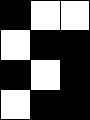
\includegraphics[width=.35\textwidth]{3outex.png}
		\caption{Graphical representation}
		\label{subfig:3outexgraph}
	\end{subfigure}
	\caption{Transposed and truncated matrix and associated visualization.}
	\label{fig:data+vis}
\end{figure}\noindent
The representation of the matrix in \ref{subfig:3outexgraph} is an example of 
the method we will use to depict matrices containing real values.

\subsubsection{Target Data}
\label{subsubsec:targetdata}
As described in \ref{subsec:generation}, we save the adjacency matrix 
corresponding to the generator along with the simulated spiking files. When an 
adjacency matrix is loaded into the target dataset for training a model, we 
flatten it, from $(n \times n)$ to $(1 \times n^2)$. This allows us to directly 
compare our targets to the outputs of the model, which will be of the same 
dimensionality.

\subsection{Generalizability}
\label{subsec:hotswap}
In most ANN implementations, feeding various data with the same label attached 
to it results in the network learning to ignore the input data and always return 
the desired label, rendering it useless. However, due to the unique structure of 
our model, this sort of overfitting is impossible.\footnote{See 
\ref{subsec:n-independence}} Therefore, we must merely construct a suitably 
representative generator network, meaning that it contains all of the 
inter-neuron relationships we expect to see in the data we ultimately feed in to 
test.

\section{Architecture}
We will first describe the architecture in terms that, while accurate on the 
macro level, do not fully reflect the actual transformations occuring in the 
implemented model. We will then proceed to a mathematically representative 
version, leaving explanation of the batched version of the model to APPENDIX 
SECTION.

\subsection{Structure \& Computation Details}
\subsubsection{Dimensionality-defining Variables}
Only two values characterize the matrices and transitions involved in the model.  
They are as follows:
\begin{description}
	\item \textit{b}: The number of steps of input data the model considers in a 
		given segment of data.
	\item \textit{d}: The length of the vectors characterizing each potential 
		connection \textit{ij}. This restricts the maximum information about 
		each potential neuron pair that the model can maintain across layer 
		transitions.
\end{description}
We determined effective values for these parameters through experimentation.

While we use the number of nodes in the generator graph, \textit{n}, to 
calculate summations and averages, the structure of our calculations is such 
that no aspects of the model are defined in terms of \textit{n}.

\subsubsection{Omitted Details}
An elementwise activation function\footnote{SEE NN PRINCIPLES} is applied to the 
matrix outputs from each layer. While this is crucial to network function, our 
primary focus in this section is the underlying principles and mathematical 
expressions thereof, and activation is somewhat trivial in comparison. For 
details on the activation functions used, see \ref{sec:activation}.

\subsection{Conceptual Model}
\label{subsec:conceptualmodel}
The operations we describe here represent a per-edge approach to our 
architecture; i.e., the layer transitions are defined in terms of calculations 
applied to single pairs of nodes, as opposed to the whole-matrix operations that 
the architecture as implemented relies on.

\subsubsection{First Transition}
To generate the first layer of the network, we inspect every pair of neurons in 
the input data. Since no pair of neurons is distinguishable from another, the 
comparison applied is the same in all cases: we apply the same convolutional 
filter to all pairs. We achieve this by concatenating the spike train of each 
neuron \textit{i} individually with every other neuron \textit{j}, then 
multiplying by a matrix $\mathbb{W}$ of dimensionality $(d \times 2b)$. To this 
product we add a bias vector, $\mathbb{B}$, of dimensionality $(d \times 1)$.

$\mathbb{W}$ is trained on, and thus the comparison of each pair of spike trains 
is left up to the network. The transition appears as follows, where $\underset{b 
\times 1}{\mathbb{I}_x}$ is the input column at \textit{x}:
\[
	\mathlarger\forall i,j \mid 0 \leq i,j < n: \underset{d \times 
	1}{d_{ij}^\prime} = \underset{d \times 2b}{\mathbb{W}} \times 
	\left(\frac{\mathbb{I}_i}{\mathbb{I}_j}\right) + \underset{d \times 
	1}{\mathbb{B}}
\]
This leaves us with $n^2$ \textit{d}-vectors, each characterizing one potential 
edge \textit{ij}.

\subsubsection{Locality Layer}
In this layer, we incorporate information from all nodes potentially adjacent to 
each edge \textit{ij}. From our previous layer, we have a matrix of shape $(d 
\times n^2)$ that we will refer to as $\mathbb{D}^{\prime}$, but it will be 
useful to keep in mind an alternate representation of that matrix, one in three 
dimensions, which we shall refer to as $\mathbb{D}_N^{\prime}$. This 
transformation is demonstrated in \figref{fig:transform}.

\begin{figure}[H]
	\centering
	\begin{tikzpicture}
	    \pgfmathsetmacro{\n}{20}
	    \pgfmathsetmacro{\t}{40}
	    \pgfmathsetmacro{\d}{12}
	    \pgfmathsetmacro{\scale}{.07}
		\pic at (2,-1) {annotated cuboid={width=\n*4, height=3, depth=\d, xlabel=n, 
		ylabel=1, zlabel=d, scale=\scale}};
	    \node at (3.7,-1) {\scalebox{2}{$\Leftrightarrow$}};
		\pic at (6.8,-.27) {annotated cuboid={width=\n, height=\n, depth=\d, 
	xlabel=n, ylabel=n, zlabel=d, scale=\scale}};
		\node at (-.8, -3)  {\scalebox{1.5}{$\mathbb{D}^{\prime}$}};
		\node at (6.3, -3) {\scalebox{1.5}{$\mathbb{D}_N^{\prime}$}};
	\end{tikzpicture}
	\caption{Relationship between $\mathbb{D}^{\prime}$ and 
		$\mathbb{D}^{\prime}_N$.}
	\label{fig:transform}
\end{figure}\noindent
Consider some $d_{ij}^{\prime}$ in $\mathbb{D}^{\prime}_N$. Then we can say the 
following:
\begin{enumerate}
	\item $d_{ij}^{\prime}$ represents the connection from \textit{j} to 
		\textit{i} as it may or may not exist in this network, in the form of 
		\textit{d} values of indeterminate meaning
	\item $\mathlarger\forall k \mid 0 \leq k < n$, $d_{jk}^{\prime}$ represents 
		a potential input to \textit{j}
	\item $\mathlarger\forall k \mid 0 \leq k < n$, $d_{ki}^{\prime}$ represents 
		a potential output from \textit{i}
\end{enumerate}
In our determination of the presence or absence of a connection from \textit{j} 
to \textit{i}, we wish to incorporate information from these potentially 
connected nodes; i.e., these inputs and outputs represent potential neighbors in 
terms of graph locality. To achieve this, we perform the following 
computations\footnote{Actually, it's much more elegant.} for each $\underset{d 
\times 1}{d_{ij}}$:
\begin{minipage}{\textwidth}
\begin{subequations}
	\centering
	\begin{align}
		\label{eq:ID}
		\underset{d \times 1}{\mathbb{I}} &= \frac{1}{n} \sum_{k=0}^{n-1} 
		d_{jk}^{\prime} & \underset{d \times 1}{\mathbb{O}} &= \frac{1}{n} 
		\sum_{k=0}^{n-1} d_{ki}^{\prime}\\
		\label{eq:IDOD}
		\underset{d \times 1}{\mathbb{I_D}} &= \underset{d \times 
			d}{\mathbb{W}_{in}^\prime} \times \left(\mathbb{I} \odot 
		d_{ij}^{\prime}\right) & \underset{d \times 1}{\mathbb{O_D}} &= 
		\underset{d \times d}{\mathbb{W}_{out}^\prime} \times \left(\mathbb{O} 
		\odot d_{ij}^{\prime}\right)
	\end{align}
	\text{Here we arrive at the output, $d_{ij}^{\prime\prime}$:}
	\begin{equation}
		\underset{d \times 1}{d_{ij}^{\prime\prime}} = \underset{d \times 
		2d}{\mathbb{W}_{tot}^\prime} \times 
		\left(\frac{\mathbb{I_D}}{\mathbb{O_D}}\right) + \underset{d \times 
		1}{\mathbb{B}^\prime}
		\label{eq:dijO} 
	\end{equation}
\end{subequations}
Conceptually, in \eqref{eq:ID} we first average all potential inputs to and 
outputs from potential edge \textit{ij}. Then, we compute an entrywise product 
($\odot$) of these vectors with the vector describing the edge in question, 
$d_{ij}^{\prime}$. While we have integrated locality data into the results thus 
far, the network has not been allowed any processing over the resultant data, 
which we rectify by multiplying the input and output vectors with separate 
dimensionality-preserving $(d \times d)$ matrices. We thus arrive at 
\eqref{eq:IDOD}, with vectors $\mathbb{I_D}$ and $\mathbb{O_D}$ representing 
edge \textit{ij} with inputs and outputs, respectively, taken into 
consideration. In \eqref{eq:dijO}, we arrive at $d_{ij}^{\prime\prime}$ by 
multiplying a third weight matrix by the vertical concatenation of 
$\mathbb{I_D}$ and $\mathbb{O_D}$.  This matrix, $\mathbb{W}_{tot}^\prime$, 
allows the network to optimize for whichever elements in $\mathbb{I_D}$ and 
$\mathbb{O_D}$ are most important in the prediction of \textit{ij}.  
Additionally, a bias vector, $\mathbb{B}^\prime$, is added to this product, and 
at this point we have $d_{ij}^{\prime\prime}$ as it will be seen by the next 
layer of the network.\footnotemark
%The three matrices involved, $\mathbb{W}_{in}^\prime$, 
%$\mathbb{W}_{out}^\prime$, and $\mathbb{W}_{tot}^\prime$, are trained on by the 
%optimizer\footnote{SEE OPTIMIZER SECION IN TRAINING}, allowing the model to 
%learn optimal processing and combinations to facilitate predictions.
\end{minipage}
\footnotetext{Disregarding activation}

Our concatenation approach in \eqref{eq:dijO} stands in contrast to the strategy 
taken in \eqref{eq:IDOD}, where integration of the input and output data is 
forced via entrywise product computation. While we considered the same 
concatenation process for use in \eqref{eq:IDOD}, the apparent difficulty of 
integrating the calculated locality data into the prediction of \textit{ij} led 
the model to rapidly adapt its weight matrices to ignore the locality portion of 
the data.  For more discussion on this difficulty, see TRAINING SECTION.

Note again that none of the computations involved in this layer are dependent on 
\textit{n}; as the summations are averaged, the values contained in their 
resultant vectors will be of similar magnitude for any number of neurons under 
consideration. After executing this algorithm for each $d_{ij}^{\prime}$, we are 
left with another $(d \times n^2)$ output matrix, $\mathbb{D}^{\prime\prime}$.

\subsubsection{Final Transition}
The shift from $(d \times n^2)$ is comparatively simple, being only a 
dimensionality reduction:
\begin{equation}
	\mathlarger\forall d_{ij}^{\prime\prime} \in \mathbb{D}^{\prime\prime}:
	\underset{1 \times 1}{d_{ij}^f} = \underset{1 \times d}{\mathbb{W}^f} \times 
	\underset{d \times 1}{d_{ij}^{\prime\prime}}
\end{equation}
This leaves us with a $(1 \times n^2)$ matrix, which, following application of 
an activation function as defined in \ref{subsec:finalactivation} and 
transposition to $(n \times n)$, we treat as the adjacency matrix of the 
generator associated with the input data.

\subsection{Matrix Model}
\label{subsec:matmodel}
While the processes defined in \ref{subsec:conceptualmodel} are accurate 
representations of the operations undertaken in our model, they are generally 
defined in terms of individual vectors, with iteration over all vectors 
necessarily implied. This does not take advantage of the computational abilities 
of modern GPU computing, and, if implemented as such, would render training 
times astronomical. Therefore, we create a version of our model executed 
entirely in terms of matrix operations, ideal for GPU execution.

\subsubsection{First Layer}
\label{subsubsec:matfirstlayer}
In the first layer, we wish to compare each input vector against every input 
vector by way of concatenation and matrix multiplication to reduce 
dimensionality. To achieve this via matrix operations is fairly simple. We first 
define two helper matrices:
\begin{align*}
	\underset{n \times n^2}{\mathbb{E}} &= \begin{bmatrix}
			\underset{1 \times n}{\mathbbm{1}} & \dots & 0\\
			\vdots & \ddots & \vdots \\
		0 & \dots & \underset{1 \times n}{\mathbbm{1}} \end{bmatrix}\\
		\underset{n \times n^2}{\mathbb{T}} &= \begin{bmatrix}
	I_n & \mid & \dots & \mid I_n \end{bmatrix}
\end{align*}
With $\underset{b \times n}{\mathbb{I}}$ as our input data, the first layer 
transition is as follows:
\begin{equation}
	\underset{d \times n^2}{\mathbb{D}^\prime} = \underset{d \times 
	2b}{\mathbb{W}}
	\left(\frac{\mathbb{I}\times\mathbb{E}}{\mathbb{I}\times\mathbb{T}}\right) + 
	\left(\underset{d \times 1}{\mathbb{B}}\times\underset{1 \times 
	n^2}{\mathbbm{1}}\right)
\end{equation}
\paragraph{Example}
Consider the a model for which $b=3$ and $n=2$. Suppose that we have the 
following input matrix: 
\[ 
	\mathbb{I} = \begin{bmatrix} 1 & 1\\ 1 & 0\\ 0 & 1\end{bmatrix}
\]
Then our helper matrices would appear as such:
\[
	\mathbb{E} = \begin{bmatrix}
		1 & 1 & 0 & 0\\
		0 & 0 & 1 & 1
	\end{bmatrix}
	\hspace{2em}
	\mathbb{T} = \begin{bmatrix}
		1 & 0 & 1 & 0\\
	0 & 1 & 0 & 1 \end{bmatrix}
\]
And our matrix stack:
\[
	\mathbb{I} = \begin{bmatrix} 1 & 1\\ 1 & 0\\ 0 & 1\end{bmatrix}
	\hspace{3em}
	\frac{\mathbb{I} \times \mathbb{E}}{\mathbb{I} \times \mathbb{T}} = 
	\begin{bmatrix}
		1 & 1 & 1 & 1\\
		1 & 1 & 0 & 0\\
		0 & 0 & 1 & 1\\
		1 & 1 & 1 & 1\\
		1 & 0 & 1 & 0\\
		0 & 1 & 0 & 1
	\end{bmatrix}
\]
Thus, over all of the columns in the resulting stack, every vector in 
$\mathbb{I}$ is paired with all such vectors, including itself.

\subsubsection{Locality Layer}
\label{subsubsec:matconvlayer}
In the conceptual model, there are two averages of sums involved in processing 
each vector in $\mathbb{D}^\prime$; one over the horizontal axis of 
$\mathbb{D}^\prime_N$, and the other over the vertical axis. These can be found 
in \eqref{eq:ID}. Consider two vectors $d_{ij}, d_{il} \in \mathbb{D}^\prime_N$.  
For both of these vectors, the average input vector is the same, its calculation 
being only dependent on the first coordinate, $i$. The inverse holds for vectors 
with the same second coordinate. Thus we see that these calculations need only 
be performed once for each $k \in [0,n)$. Considering the $(d \times n^2)$ 
representation of the current data matrix $\mathbb{D}^\prime$, the `vertical' 
summation of column \textit{i} appears as such:
\[
	\mathbb{O} = \sum_k d^\prime_{ki} = \mathbb{D}^\prime_{0+i} + 
	\mathbb{D}^\prime_n + \mathbb{D}^\prime_{2n + i} + \dots + 
	\mathbb{D}^\prime_{(n-1)n + i}
\]
This is the inverse of the tile operation executed by $\mathbb{T}$ in the first 
layer, and that same matrix allows us to compute all outputs to all edges 
simultaneously:
\[
	\underset{d \times n}{\mathbb{O}} = \frac{1}{n} \left(\mathbb{D}^\prime 
	\times \mathbb{T}^\top\right)
\]
Similarly, to calculate the sum of row j in $\mathbb{D}^\prime_N$:
\[
	\mathbb{I} = \sum_k d^\prime_{jk} = \sum_{l=j}^{j + n-1} \mathbb{D}^\prime_l
\]
This is the inverse of the expand operation executed by $\mathbb{E}$, and once 
again we can use that same matrix to compute all edge inputs simultaneously:
\[
	\underset{d \times n}{\mathbb{I}} = \frac{1}{n}\left(\mathbb{D}^\prime 
	\times \mathbb{E}^\top \right)
\]
These operations allow us to avoid ever transposing $\mathbb{D}^\prime$, instead 
allowing us to work directly on it.

For both $\mathbb{I}$ and $\mathbb{O}$, we still need to pair the vectors within 
with the appropriate vector in $\mathbb{D}^\prime$. To accomplish this, we must 
expand both matrices to $(d \times n^2)$. 

For some vector $\mathbb{I}_x$, we wish to pair it with all vectors $d_{kx} \in 
\mathbb{D}^\prime_N \mid k \in [0,n)$. In terms of $\mathbb{D}^\prime$, these 
vectors map to $\mathbb{D}^\prime_{kn+x}$; i.e., we wish to create a matrix into 
which we distribute a given vector in $\mathbb{I}$ \textit{n} times, \textit{n} 
columns apart. Once again, we already have a matrix specifically capable of this 
operation: $\mathbb{T}$.  Similarly, we wish to pair any given vector 
$\mathbb{O}_x$ with all vectors ${d_{xk} \in \mathbb{D}^\prime_N \mid k \in 
[0,n)}$, which correspond with $\mathbb{D}^\prime_{xn + k}$: for each vector in 
$\mathbb{O}$, we broadcast it into a $(d \times n^2)$ matrix such that it 
repeats \textit{n} times. Yet again, an established matrix will complete this 
task: $\mathbb{E}$.

Thus our intermediary steps for this layer are quite similar to \eqref{eq:IDOD}:
\begin{subequations}
	\centering
	\begin{align}
		\underset{d \times n^2}{\mathbb{I_D}} &= \underset{d \times 
		d}{\mathbb{W}_{in}^\prime} \times \left(\left(\mathbb{I} \times 
	\mathbb{T}\right) \odot \mathbb{D}^\prime\right) & \underset{d \times 
n^2}{\mathbb{O_D}} &= \underset{d \times d}{\mathbb{W}_{out}^\prime} \times 
\left(\left(\mathbb{O} \times \mathbb{E}\right) \odot \mathbb{D}^\prime\right)
	\end{align}
	\text{We arrive at the matrix expression of the locality layer:}
	\begin{equation}
		\underset{d \times n^2}{\mathbb{D}^{\prime\prime}} = \underset{d \times 
			d}{\mathbb{W}_{tot}^\prime} \times 
			\left(\frac{\mathbb{I_D}}{\mathbb{O_D}}\right) + \left(\underset{d 
			\times 1}{\mathbb{B}^\prime} \times \underset{1 \times 
	n^2}{\mathbbm{1}}\right)
	\end{equation}
\end{subequations}


\subsubsection{Final Layer}
\label{subsubsec:matfinallayer}

\subsection{\textit{n}-independence}
\label{subsec:nindependence}
\subsubsection{Trainable Values}
Between all of the operations defined in \ref{subsec:matmodel} (and equivalently 
in \ref{subsec:conceptualmodel}), the following matrices are the only trainable 
values:
\subparagraph{First Layer}
\begin{itemize}
	\item[$\ubb{W}{d}{2b}$:] weight matrix used to merge columns of input data
	\item[$\ubb{B}{d}{1}$:] bias vector added to every $d_{ij}^\prime$
\end{itemize}

\subparagraph{Convolutional Layer}
\begin{itemize}
	\item[$\underset{d \times d}{\mathbb{W}_{in}^\prime}$:] weight matrix used 
		to process data entering an edge
	\item[$\underset{d \times d}{\mathbb{W}_{out}^\prime}$:] weight matrix used 
		to process data exiting an edge
	\item[$\underset{d \times 2d}{\mathbb{W}_{tot}^\prime}$:] weight matrix used 
		to merge the data produced by $\underset{d \times 
			d}{\mathbb{W}_{out}^\prime}$ and $\underset{d \times
			d}{\mathbb{W}_{in}^\prime}$
	\item[$\underset{d \times 1}{\mathbb{B}^\prime}$:] bias vector added to 
		every $d_{ij}^{\prime\prime}$
\end{itemize}

\subparagraph{Final Layer}
\begin{itemize}
	\item[$\underset{1 \times d}{\mathbb{W}}^f$:] weight matrix used to collapse 
		previous outputs into one value
\end{itemize}
\subsubsection{Implications}
As noted previously, none of these matrices are dependent on \textit{n}.  
Furthermore, even in the matrix model (\ref{subsec:matmodel}), the weight 
matrices operate individually on each \textit{ij} vector, and the same bias is 
added to each vector.  Because the network is not provided any trainable 
\textit{n}-scale values, all calculation and training is done per node pair.  
This obviates the typical neural network problem of overfitting to its training 
dataset to the point it simply memorizes appropriate outputs.\footnote{See 
\ref{sec:overfitting}} Additionally, this allows for application of a trained 
model to data produced by generators of a different size than those used to 
train the model. Because our model operates entirely on local graph features, 
the only requirement for such an application is that the training data contain a 
set of features also representative of the new data.
